\documentclass[aspectratio=43]{beamer}
% \documentclass[aspectratio=169]{beamer}

% Title --------------------------------------------
\title{\huge Conflict termination and\\postwar politics}
\author{Francisco Villamil}
\date{War, peace, and political violence\\UC3M, Fall 2022}

%%% NOTE -- CHECK THIS: https://github.com/paulgp/beamer-tips


%%% Building heavily on https://github.com/kylebutts/templates

% xcolor, define them
\usepackage{xcolor}

% TEXT COLORS
\definecolor{red}{HTML}{9a2515}
\definecolor{yellow}{HTML}{EBC944}
\definecolor{asher}{HTML}{555F61}
\definecolor{jet}{HTML}{131516}

% THEME COLORS
\definecolor{accent}{HTML}{107895}
\definecolor{accent2}{HTML}{9a2515}

% Color commands
\newcommand\red[1]{{\color{red}#1}}
\newcommand\yellow[1]{{\color{yellow}#1}}
\newcommand\asher[1]{{\color{asher}#1}}

\newcommand\BGred[1]{{\colorbox{red!80!white}{#1}}}
\newcommand\BGyellow[1]{{\colorbox{yellow!80!white}{#1}}}
\newcommand\BGasher[1]{{\colorbox{asher!80!white}{#1}}}

\renewcommand<>{\BGyellow}[1]{\only#2{\beameroriginal{\BGyellow}}{#1}}

% Appendix numbering
\usepackage{appendixnumberbeamer}

% Beamer Options -------------------------------------

% Background
\setbeamercolor{background canvas}{bg = white}

% Change text margins
\setbeamersize{text margin left = 25pt, text margin right = 15pt}

% \alert
\setbeamercolor{alerted text}{fg = accent2}

% Frame title
\setbeamercolor{frametitle}{bg = white, fg = jet}
\setbeamercolor{framesubtitle}{bg = white, fg = accent}
\setbeamerfont{framesubtitle}{size = \small, shape = \itshape}

% Block
\setbeamercolor{block title}{fg = white, bg = accent2}
\setbeamercolor{block body}{fg = jet, bg = jet!10!white}

% Title page
\setbeamercolor{title}{fg = jet}
\setbeamercolor{subtitle}{fg = accent}

%% Custom \maketitle and \titlepage
\setbeamertemplate{title page}
{
    \begin{centering}
      % \vspace{20mm}
      {\Large \usebeamerfont{title}\usebeamercolor[fg]{title}\inserttitle}\\ \vskip0.25em%
      \ifx\insertsubtitle\@empty%
      \else%
        {\usebeamerfont{subtitle}\usebeamercolor[fg]{subtitle}\insertsubtitle\par}%
      \fi%
      {\vspace{10mm}\insertauthor}\\
      \ifx\insertinstitute\@empty%
      \else%
        {\vspace{5mm}\color{asher}\scriptsize{\insertinstitute}}
      \fi%
      {\color{asher}\small{\insertdate}}\\
    \end{centering}
}

% Table of Contents
\setbeamercolor{section in toc}{fg = accent!70!jet}
\setbeamercolor{subsection in toc}{fg = jet}

% Button
\setbeamercolor{button}{bg = accent}

% Remove navigation symbols
\setbeamertemplate{navigation symbols}{}

% Table and Figure captions
\setbeamercolor{caption}{fg=jet!70!white}
\setbeamercolor{caption name}{fg=jet}
\setbeamerfont{caption name}{shape = \itshape}

% Put slide number / total slides at the bottom right
\makeatother
\makeatletter
\setbeamertemplate{footline} %{\hfill\insertframenumber/\inserttotalframenumber}
{%
  \leavevmode%
  \hbox{
  \begin{beamercolorbox}[wd=\paperwidth,ht=2.5ex,dp=1.125ex,leftskip=.3cm,rightskip=.3cm plus1fil]{footlinecolor}%
    \color{asher}{\hfill\insertframenumber/\inserttotalframenumber}
  \end{beamercolorbox}}%
  \vskip0pt%
}
\makeatother
\makeatletter

% Bullet points

%% Fix left-margins
\settowidth{\leftmargini}{\usebeamertemplate{itemize item}}
\addtolength{\leftmargini}{\labelsep}

%% enumerate item color
\setbeamercolor{enumerate item}{fg = accent}
\setbeamerfont{enumerate item}{size = \small}
\setbeamertemplate{enumerate item}{\insertenumlabel.}

%% itemize
\setbeamercolor{itemize item}{fg = accent!70!white}
\setbeamerfont{itemize item}{size = \small}
\setbeamertemplate{itemize item}[circle]
\setlength{\itemsep}{0pt plus 6pt}

%% right arrow for subitems
\setbeamercolor{itemize subitem}{fg = accent!60!white}
\setbeamerfont{itemize subitem}{size = \small}
\setbeamertemplate{itemize subitem}{$\rightarrow$}

\setbeamertemplate{itemize subsubitem}[square]
\setbeamercolor{itemize subsubitem}{fg = jet}
\setbeamerfont{itemize subsubitem}{size = \small}

% References

%% Bibliography Font, roughly matching aea
\setbeamerfont{bibliography item}{size = \footnotesize}
\setbeamerfont{bibliography entry author}{size = \footnotesize, series = \bfseries}
\setbeamerfont{bibliography entry title}{size = \footnotesize}
\setbeamerfont{bibliography entry location}{size = \footnotesize, shape = \itshape}
\setbeamerfont{bibliography entry note}{size = \footnotesize}

\setbeamercolor{bibliography item}{fg = jet}
\setbeamercolor{bibliography entry author}{fg = accent!60!jet}
\setbeamercolor{bibliography entry title}{fg = jet}
\setbeamercolor{bibliography entry location}{fg = jet}
\setbeamercolor{bibliography entry note}{fg = jet}

%% Remove bibliography symbol in slides
\setbeamertemplate{bibliography item}{}





% Links ----------------------------------------------

\usepackage{hyperref}
\hypersetup{
  colorlinks = true,
  linkcolor = accent,
  filecolor = accent,
  urlcolor = accent,
  citecolor = accent,
}


% Line spacing --------------------------------------
\usepackage{setspace}
\setstretch{1.2}


% \begin{columns} -----------------------------------
\usepackage{multicol}


% % Fonts ---------------------------------------------
% % Beamer Option to use custom fonts
% \usefonttheme{professionalfonts}
%
% % \usepackage[utopia, smallerops, varg]{newtxmath}
% % \usepackage{utopia}
% \usepackage[sfdefault,light]{roboto}
%
% % Small adjustments to text kerning
% \usepackage{microtype}



% Remove annoying over-full box warnings -----------
\vfuzz2pt
\hfuzz2pt


% Table of Contents with Sections
\setbeamerfont{myTOC}{series=\bfseries, size=\Large}
\AtBeginSection[]{
        \frame{
            \frametitle{Roadmap}
            \tableofcontents[current]
        }
    }


% References ----------------------------------------
\usepackage[
    citestyle= authoryear,
    style = authoryear,
    natbib = true,
    backend = biber
]{biblatex}

% Smaller font-size for references
\renewcommand*{\bibfont}{\small}

% Remove "In:"
\renewbibmacro{in:}{}

% Color citations for slides
\newenvironment{citecolor}
    {\footnotesize\begin{color}{accent2}}
    {\end{color}}

\newcommand{\citetcolor}[1]{{\footnotesize\textcolor{asher}{\citet{#1}}}}
\newcommand{\citepcolor}[1]{{\footnotesize\textcolor{asher}{\citep{#1}}}}

% Tables -------------------------------------------
% Tables too big
% \begin{adjustbox}{width = 1.2\textwidth, center}
\usepackage{adjustbox}
\usepackage{array}
\usepackage{threeparttable, booktabs, adjustbox}

% Fix \input with tables
% \input fails when \\ is at end of external .tex file

\makeatletter
\let\input\@@input
\makeatother

% Tables too narrow
% \begin{tabularx}{\linewidth}{cols}
% col-types: X - center, L - left, R -right
% Relative scale: >{\hsize=.8\hsize}X/L/R
\usepackage{tabularx}
\newcolumntype{L}{>{\raggedright\arraybackslash}X}
\newcolumntype{R}{>{\raggedleft\arraybackslash}X}
\newcolumntype{C}{>{\centering\arraybackslash}X}

% Figures

% \imageframe{img_name} -----------------------------
% from https://github.com/mattjetwell/cousteau
\newcommand{\imageframe}[1]{%
    \begin{frame}[plain]
        \begin{tikzpicture}[remember picture, overlay]
            \node[at = (current page.center), xshift = 0cm] (cover) {%
                \includegraphics[keepaspectratio, width=\paperwidth, height=\paperheight]{#1}
            };
        \end{tikzpicture}
    \end{frame}%
}

% subfigures
\usepackage{subfigure}


% Highlight slide -----------------------------------
% \begin{transitionframe} Text \end{transitionframe}
% from paulgp's beamer tips
\newenvironment{transitionframe}{
    \setbeamercolor{background canvas}{bg=accent!60!black}
    \begin{frame}\color{accent!10!white}\LARGE\centering
}{
    \end{frame}
}


% Table Highlighting --------------------------------
% Create top-left and bottom-right markets in tabular cells with a unique matching id and these commands will outline those cells
\usepackage[beamer,customcolors]{hf-tikz}
\usetikzlibrary{calc}
\usetikzlibrary{fit,shapes.misc}

% To set the hypothesis highlighting boxes red.
\newcommand\marktopleft[1]{%
    \tikz[overlay,remember picture]
        \node (marker-#1-a) at (0,1.5ex) {};%
}
\newcommand\markbottomright[1]{%
    \tikz[overlay,remember picture]
        \node (marker-#1-b) at (0,0) {};%
    \tikz[accent!80!jet, ultra thick, overlay, remember picture, inner sep=4pt]
        \node[draw, rectangle, fit=(marker-#1-a.center) (marker-#1-b.center)] {};%
}


\begin{document}

% ------------------------------------------
\begin{frame}
  \titlepage
\end{frame}
% ------------------------------------------

% ----------------------------------------------------
\begin{frame}
\frametitle{Not all is written when a war breaks out}
\centering

\begin{itemize}[<+->]
  \item When do civil wars end?
  \item How do they end?
  \item Why do they break out again?
  \item How can we enforce peace?
\end{itemize}

\end{frame}
% ----------------------------------------------------

% ----------------------------------------------------
\begin{frame}
\frametitle{The \textit{duration} of civil wars}
\centering

\begin{itemize}[<+->]
  \item Why do some wars last so much longer than others? {\scriptsize (Fearon 2004)}
  \item Two types of particularly long conflicts
  \begin{itemize}
    \item Conflicts where rebel groups receive funding from {\color{red}{contraband}} activities: diamonds, coca, opium...
    \item {\color{red}{`Sons-of-the-soil'}} conflicts: ethnic minority in the periphery against a dominant ethnic group that supports migrants into the periphery
  \end{itemize}
  \item Why?
\end{itemize}
% Balcells, L., & Kalyvas, S. N. (2014). Does Warfare Matter? Severity, Duration, and Outcomes of Civil Wars. Journal of Conflict Resolution, 58(8), 1390–1418.

\end{frame}
% ----------------------------------------------------

% ----------------------------------------------------
\begin{frame}
\frametitle{The \textit{duration} of civil wars \& commitment problems}
\centering

\begin{itemize}[<+->]
  \item Why would I stop fighting and reach a {\color{red}{\textbf{negotiated settlement}}}?
  \item Usually about the {\color{red}{incentives}} of fighting actors to negotiate or about how {\color{red}{credible}} it would be
  \item Explains the previous two types
  \begin{itemize}
    \item Wartime contraband is making me rich even if fighting is costly
    \item I'm sending migrants of my group to your region, which will increase in local power in the future
  \end{itemize}
  \item There is another explanation to sons-of-the-soil longer duration:
        ethnic exclusion $\rightarrow$ group solidarity \& mobilization $\rightarrow$ longer wars
\end{itemize}

\end{frame}
% ----------------------------------------------------

% ----------------------------------------------------
\begin{frame}
\frametitle{The \textit{duration} of civil wars \& warfare technology}
\centering

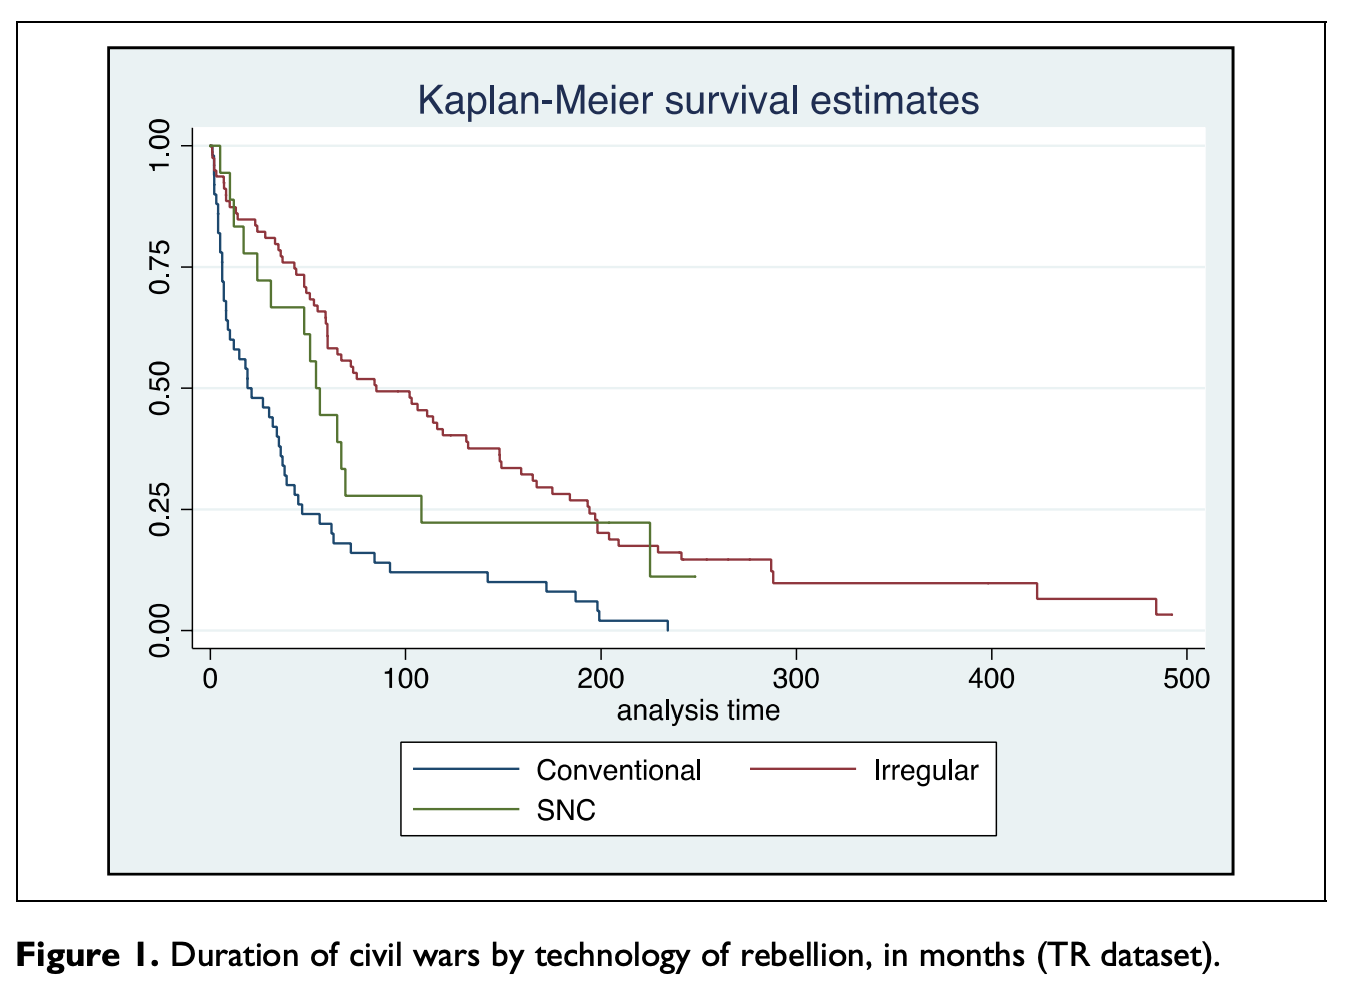
\includegraphics[width = 0.75\textwidth]{img/balcells_kalyvas_duration}

\begin{itemize}
  \visible<2>{\item Also impacts outcome: irregular wars are more likely to be won by governments and conventional wars by rebels}
\end{itemize}

{\scriptsize Balcells \& Kalyvas (2014)}

\end{frame}
% ----------------------------------------------------

% ----------------------------------------------------
\imageframe{img/ftfarc}
% ----------------------------------------------------

% ----------------------------------------------------
\begin{frame}
\frametitle{How can wars end?}
\centering

\begin{itemize}[<+->]
  \item Military victory
  \item Negotiated settlement
  \item Ceasefires
\end{itemize}

\end{frame}
% ----------------------------------------------------

% ----------------------------------------------------
\imageframe{img/cw_ends_hartzell}
% ----------------------------------------------------

% ----------------------------------------------------
\begin{frame}
\frametitle{Why the change after 1990?}
\centering

\begin{itemize}
  \item How can the international system influence incentives to negotiate?
  \item<2->[1.] Changes in external support
  \item<3->[2.] Instruments to solve the {\color{red}{credible commitment problem}}
  \begin{itemize}
    \item International Peacekeeping
    \item[] (became widespread after 1990)
  \end{itemize}
  \item<4->[]
  \item<4-> Recent trends on this?
\end{itemize}

\end{frame}
% ----------------------------------------------------

% ----------------------------------------------------
\begin{frame}
\frametitle{External peace interventions}
\centering

\begin{itemize}
  \item International organizations play a role
  \item Mediation, credible commitments, enforcing or strenghtening peace, etc
  \item Different types of interventions
\end{itemize}

\end{frame}
% ----------------------------------------------------

% ----------------------------------------------------
\begin{frame}
\frametitle{Peacekeeping, peace enforcement, peacebuilding}
\centering

\begin{itemize}[<+->]
  \item \textbf{{\color{red}{Peacekeeping:}}} deployment of international personnel to help maintain peace and security
  \item \textbf{{\color{red}{Peace enforcement:}}} the use of force to maintain peace
  \begin{itemize}
    \item Peacekeeping as `Chapter Six and a Half' (Hammarskjöld)
    \item (Chapter VI: ``pacific settlement of disputes''; C VII: ``action with respect to threats to the peace'')
  \end{itemize}
  \item \textbf{{\color{red}{Peacebuilding:}}} create the conditions so peace is self-kept
\end{itemize}

\end{frame}
% ----------------------------------------------------

% ----------------------------------------------------
\begin{frame}
\frametitle{Peacekeeping}
\centering

% \begin{minipage}{0.6\textwidth}\centering
  \begin{itemize}[<+->]
    \item Deployment of international personnel to help maintain peace and security
    \item Some include efforts to terminate violence, others only refer to post-violence actions, some include only UN-missions and other also regional organizations, ...
    \item Before 1990: few missions, focus on interstate disputes
    \item After 1990: no more deadlock in Security Council, focus on peace \textit{within} states, not between
    % \item Missions get more complicated (not only looking at troop movement, etc)
  \end{itemize}
% \end{minipage}\hfill
% \begin{minipage}{0.39\textwidth}\centering
% 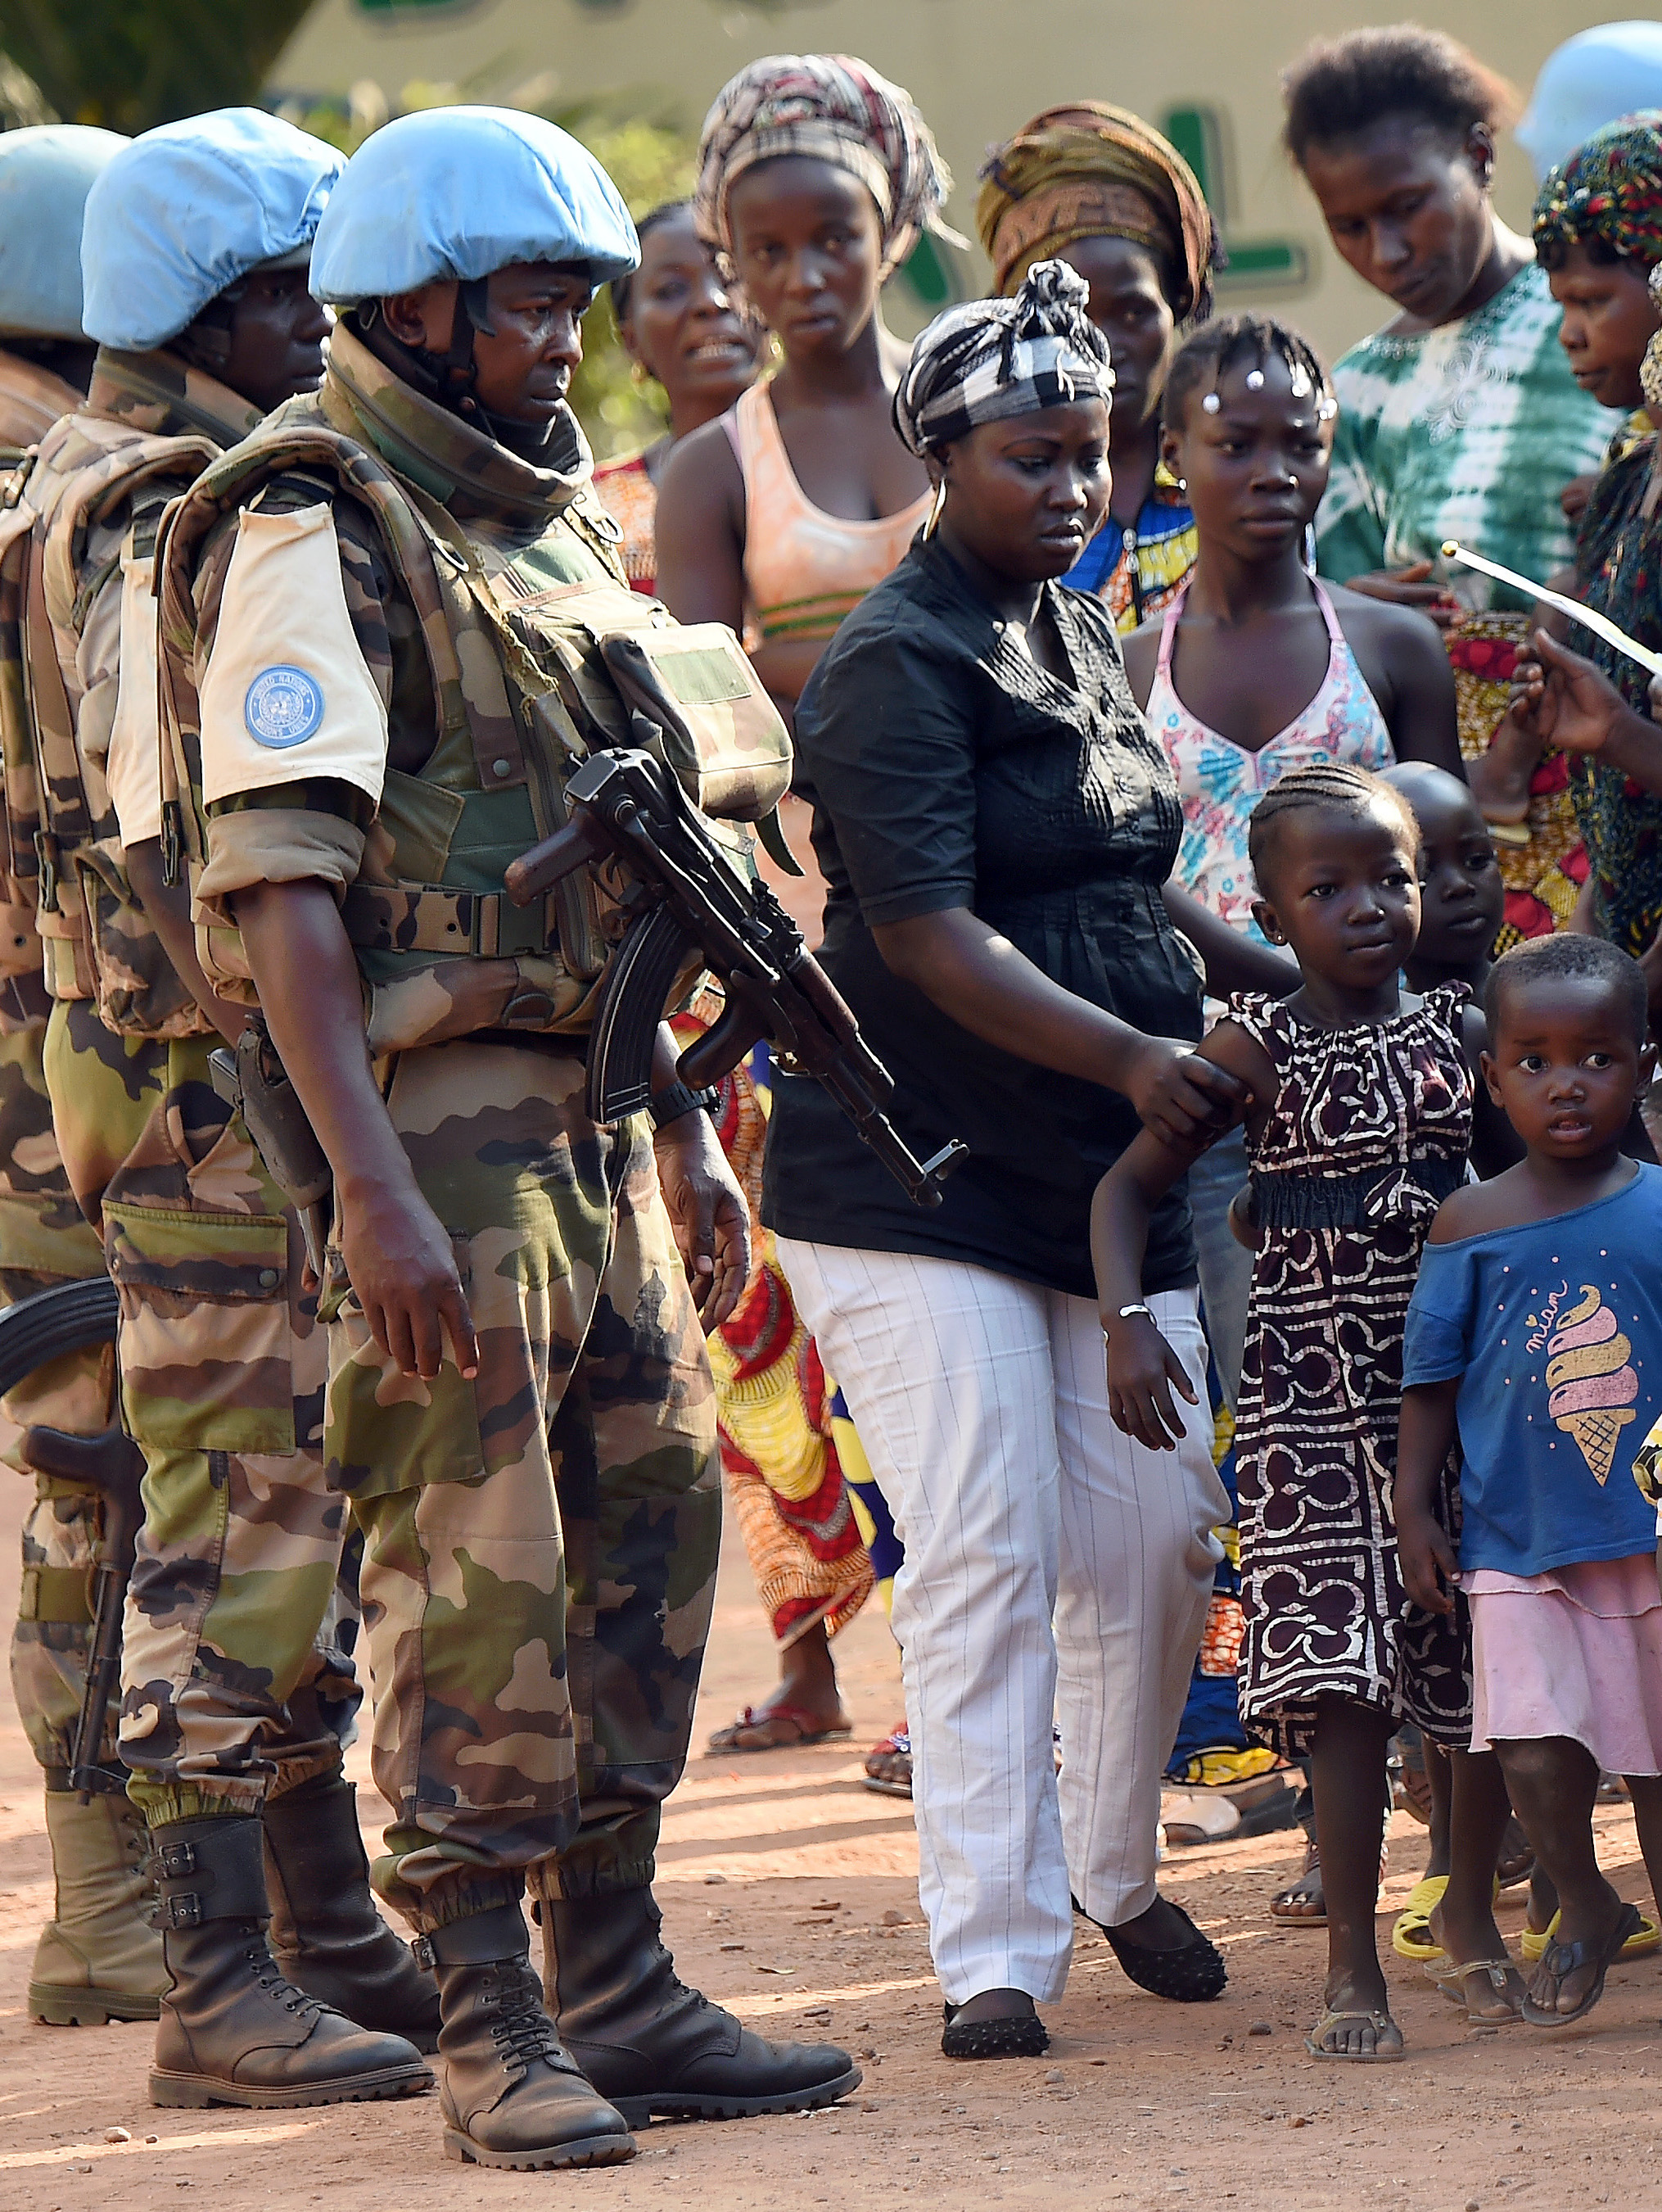
\includegraphics[width = \textwidth]{img/blue_helmets_CAR}\\
% {\small `Blue helmets' in Central African Republic}
% \end{minipage}

\end{frame}
% ----------------------------------------------------

% ----------------------------------------------------
\imageframe{img/UN_PK_troops_1947_2014}
% ----------------------------------------------------

% ----------------------------------------------------
\begin{frame}
\frametitle{Late 1990s pessimism}
\centering

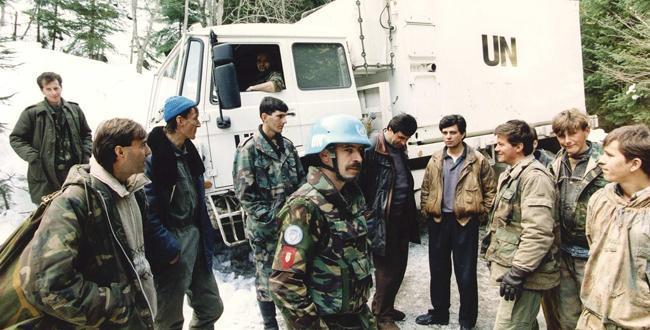
\includegraphics[width = 0.8\textwidth]{img/srebrenica-dutch-peacekeepers}\\
{\small Dutch Blue Helmets in Bosnia}

\vspace{10pt}

\begin{itemize}
  \item Srebrenica Massacre (July 1995)
  \item $>$8000 Bosniaks killed by the Bosnian Serb Army in a UN-designated ``safe area'' protected by Dutch Blue Helmets
\end{itemize}

\end{frame}
% ----------------------------------------------------

% ----------------------------------------------------
\begin{frame}
\frametitle{Late 1990s pessimism}
\centering

\begin{itemize}[<+->]
  \item On June 1993, 24 Pakistani peacekeeping soldiers were killed in Mogadishu, followed by the Battle of Mogadishu in October
  \item Big failures is Bosnia, Rwanda, Angola, etc
  \item A deep pessimism replaces the previous optimism about the role of the UN as a conflict resolution institution
  \item This pessimism was present in both theory and practice
\end{itemize}

\end{frame}
% ----------------------------------------------------

% ----------------------------------------------------
\begin{frame}
\frametitle{Late 1990s pessimism}
\centering

\begin{minipage}{0.49\textwidth}\centering
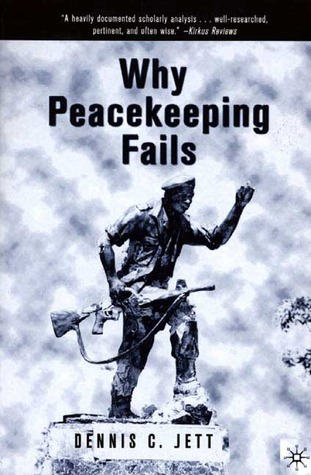
\includegraphics[width = 0.8\textwidth]{img/why-pk-fails}\\
% {\small Jett (1999)}
\end{minipage}\hfill
\begin{minipage}{0.49\textwidth}\centering
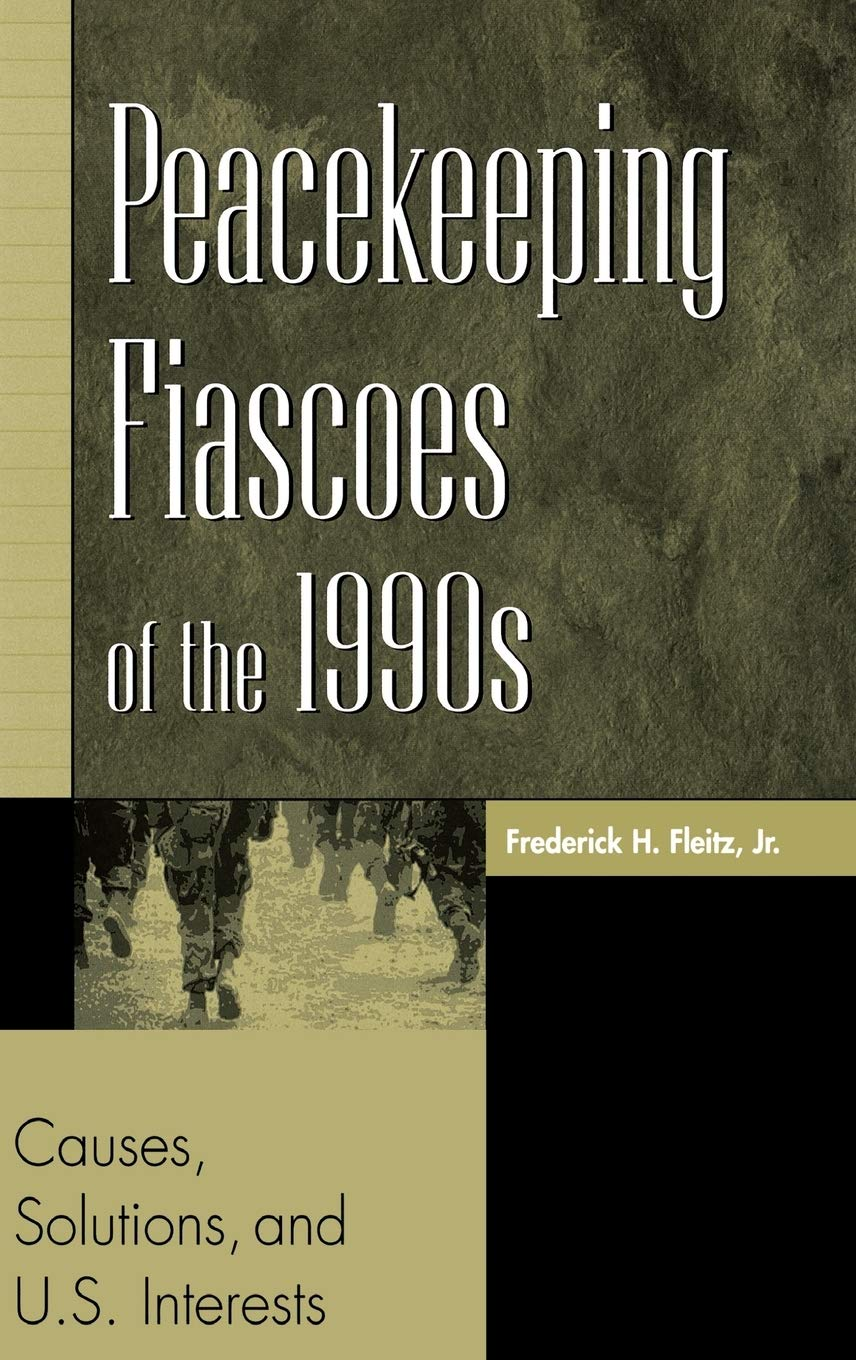
\includegraphics[width = 0.8\textwidth]{img/pk-fiascoes}\\
% {\small Fleitz (2002)}
\end{minipage}

\end{frame}
% ----------------------------------------------------

% ----------------------------------------------------
\imageframe{img/luttwak}
% {\small \textit{Foreign Affairs} 78(4), Summer 1999}
% ----------------------------------------------------

% ----------------------------------------------------
\imageframe{img/UN_PK_troops_1990_2014}
% ----------------------------------------------------

% ----------------------------------------------------
\begin{frame}
\frametitle{Does it keep peace?}
\centering

\begin{itemize}[<+->]
  \item Can we {\color{red}{study}} peacekeeping?
  \begin{itemize}
    \item What kind of missions are more effective? Does it have the same effect on battle violence than on violence against civilians? Effect on state violence vs rebel violence? (etc)
  \end{itemize}
  \item The problem: {\color{red}{\textbf{selection bias}}}
  \begin{itemize}
  \item Peacekeeping operations are not sent to a random selection of conflicts, but perhaps to the worst cases
  \item We cannot look only at the outcome of conflicts with PKO (we know that the Bosnia mission failed in protecting civilians, but do we know what would have had happened without them?)
  \end{itemize}
\end{itemize}

\end{frame}
% ----------------------------------------------------

% ----------------------------------------------------
\begin{frame}
\frametitle{New wave in the 2000s}
\centering

\begin{itemize}[<+->]
  \item Previous studies only focused on cases with PKO (hence the pessimism), new ones a bit more sophisticated
  \item Main finding: PKO are {\color{red}{{\color{red}{effective}}}}
  \item Also in practice, strong increase in PKO missions after around 2000: Kosovo, Sierra Leone, DRC...
  \item Self-critical reports on Rwanda and Bosnia, Kofi Annan had been head of the Dept of PKO, new US Ambassador, `Brahimi Report,' increased UN resources to PKO, ...
\end{itemize}

\end{frame}
% ----------------------------------------------------

% ----------------------------------------------------
\begin{frame}
\frametitle{What do we know?}
\centering

\begin{itemize}[<+->]
  \item Peace lasts longer when there are international peacekeeping troops
  \item PKO missions are effective in both civil and interstate wars
  \item PKO are effective both at creating initial peace and at sustaining it
  \item Some missions take longer to exit because of fear violence will resume (e.g. Kosovo), but PKO have been also successful at creating durable peace
  \item Many successful cases: Croatia, El Salvador, Mozambique, etc
\end{itemize}

\end{frame}
% ----------------------------------------------------

% ----------------------------------------------------
\begin{frame}
\frametitle{Where do peacekeepers go?}
\centering

\begin{itemize}[<+->]
  \item We said that PKO missions are not sent at random: they might select into the `hard cases' (or avoid very difficult conflict)
  \item What do we know about this?
  \item[1.] Interests of the permanent 5 in the UN Security Council
  \item[2.] Interests of the international community in transforming conflict-torn countries into liberal democracies
  \item[3.] In some cases, humanitarian reasons
  \item[4.] PKO usually go to the hard cases
  \item[5.] Demand from local actors
\end{itemize}

\end{frame}
% ----------------------------------------------------

% ----------------------------------------------------
\begin{frame}
\frametitle{How does peacekeeping work?}
\centering

\begin{itemize}[<+->]
  \item If local actors want to fight, they will, and if they don't want to fight, they won't
  \item So how does peacekeeping work?
  \item {\color{red}{Sustaining}} ceasefires and negotiated settlements by
  \item[1.] Raising costs of unilateral violence
  \item[2.] International observers
  \item[3.] External pressure for compliance
\end{itemize}

\end{frame}
% ----------------------------------------------------

% ----------------------------------------------------
\begin{frame}
\frametitle{Different types of peacekeeping?}
\centering

\begin{itemize}[<+->]
  \item Typical image: UN blue helmets
  \item But many other different organizations also organize PKO: EU, NATO, coalitions of states and other regional organizations (African Union and Eastern Africa Standby Force, Economic Community of West African States, etc)
  \item Also, different levels of peacekeeping
  \item[1.] Monitoring ceasefire or settlement conditions
  \item[2.] Troop deployment, buffer zone, ...
  \item[3.] Multidimensional peacekeeping (military \& civilian)
  \item[4.] Peace enforcement
\end{itemize}

\end{frame}
% ----------------------------------------------------

% ----------------------------------------------------
\begin{frame}
\frametitle{Peacebuilding strategies}
\centering

\begin{itemize}
  \item Peacebuilding strategies (avoinding conflict \textit{recurrence}) follow similar logics to the study of civil war onset
  \item<2->[1.] \textbf{{\color{red}{Greed}}-based}: postconflict peace more stable if there is economic growth
  \item<3->[2.] \textbf{{\color{red}{Opportunity}}-based}: focus on strenghtening state capacity after a conflict, and commitment problems in power-sharing
  \item<4->[3.] \textbf{{\color{red}{Grievance}}-based}: postconflict peace more stable if there are power-sharing agreements
  \item<4->[]
  \item<4-> Of all of this, power-sharing and other negotiated settlements are often part of peacebuilding strategies
\end{itemize}

\end{frame}
% ----------------------------------------------------

% ----------------------------------------------------
\begin{frame}
\frametitle{The role of power-sharing}
\centering

\begin{itemize}
  \item \BGyellow{Peace agreements} can include provisions of political, territorial, military, and economic power-sharing
  \item<2-> Each of this dimensions is different
  \item<2-> Early studies found that multi-dimensional agreements are more effective in preventing conflict recurrence
  \item<3-> However, their effect might depend on \textbf{timing} and be more problematic in cases of ethnic conflict
  \item<4-> For example: \BGyellow{Territorial power-sharing} (autonomy) seems to prevent conflict onset but not recurrence: once conflict has taken place, the commitment problem is worse and effective agreements might need government power-sharing as well
\end{itemize}

\end{frame}
% ----------------------------------------------------

% ----------------------------------------------------
\imageframe{img/southsudan1}
% ----------------------------------------------------

% ----------------------------------------------------
\imageframe{img/southsudan2}
% ----------------------------------------------------


% ----------------------------------------------------
\begin{frame}
\frametitle{The conflict \textit{trap}}
\centering

\begin{itemize}[<+->]
  \item Around half of civil war onsets are instances of conflict recurrence
  \item The main difference with explanations of `fresh' civil war onset: what happens \textit{during} the first conflict affects a second outbreak
  \item Again, different perspectives:
  \begin{itemize}
    \item {\color{red}{Grievance}}-based: postconflict peace more stable if there are power-sharing agreements
    \item {\color{red}{Greed}}-based: postconflict peace more stable if there is economic growth
    \item {\color{red}{Opportunity}}-based: focus on strenghtening state capacity after a conflict, and commitment problems in power-sharing
    \item Reality? A bit of everything
  \end{itemize}
\end{itemize}

\end{frame}
% ----------------------------------------------------

% ----------------------------------------------------
\begin{frame}
\frametitle{Is ethnic power-sharing effective?}
\centering

\begin{itemize}[<+->]
  \item Regional autonomy vs central power-sharing
  \item Effectiveness depends:
  \begin{itemize}
    \item Autonomy concessions work {\color{red}{before}} conflict outbreak
    \item But they do {\color{red}{not}} prevent {\color{red}{recurrence}}
    \item If there has already been a war, {\color{red}{central power-sharing}} needed
  \end{itemize}
\end{itemize}

\end{frame}
% ----------------------------------------------------

% ----------------------------------------------------
\imageframe{img/moro_map}
% ----------------------------------------------------

% ----------------------------------------------------
\begin{frame}
\frametitle{Moro conflict}
\centering

\begin{minipage}{0.38\textwidth}\centering
\begin{itemize}
  \item MNLF (1968)
  \item Moro Islamic Liberation Front (1977)
\end{itemize}

\end{minipage}\hfill
\begin{minipage}{0.6\textwidth}\centering
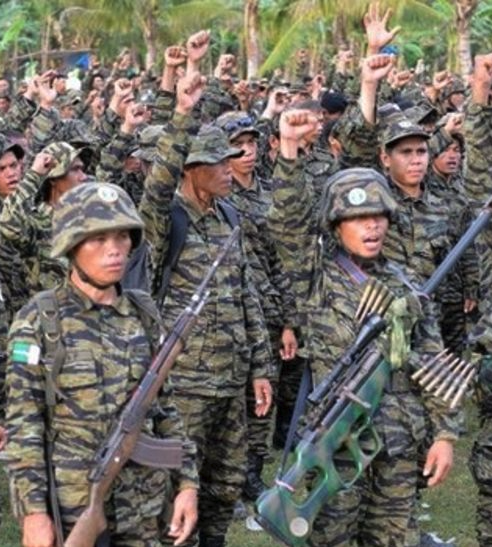
\includegraphics[width = 0.8\textwidth]{img/moro_fighters}
\end{minipage}



\end{frame}
% ----------------------------------------------------

% ----------------------------------------------------
\begin{frame}
\frametitle{1996 Final Peace Agreement (MNLF)}
\centering

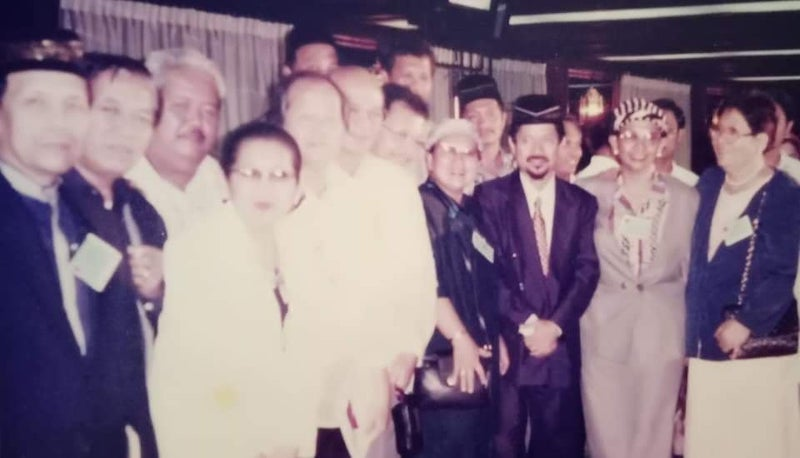
\includegraphics[width = \textwidth]{img/moro1996}

\end{frame}
% ----------------------------------------------------

% % ----------------------------------------------------
% \imageframe{img/moro3}
% % ----------------------------------------------------

% ----------------------------------------------------
\begin{frame}
\frametitle{Moro Islamic Liberation Front}
\centering

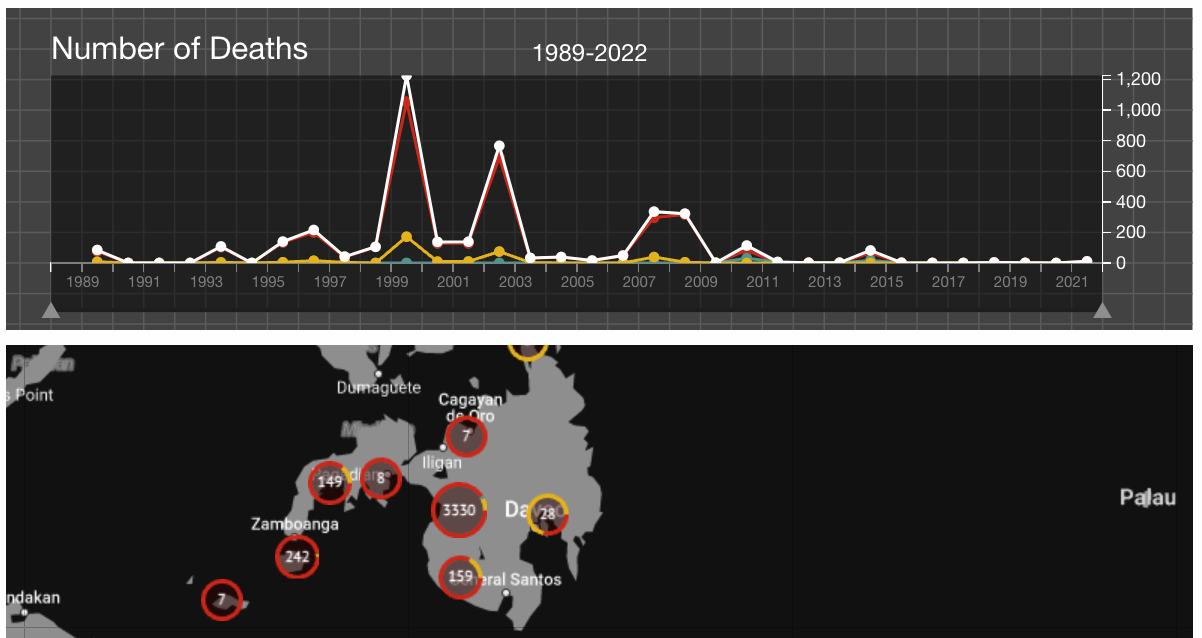
\includegraphics[width = \textwidth]{img/milf_uppsala}

\end{frame}
% ----------------------------------------------------

% ----------------------------------------------------
\begin{frame}
\frametitle{Access to central power?}
\centering

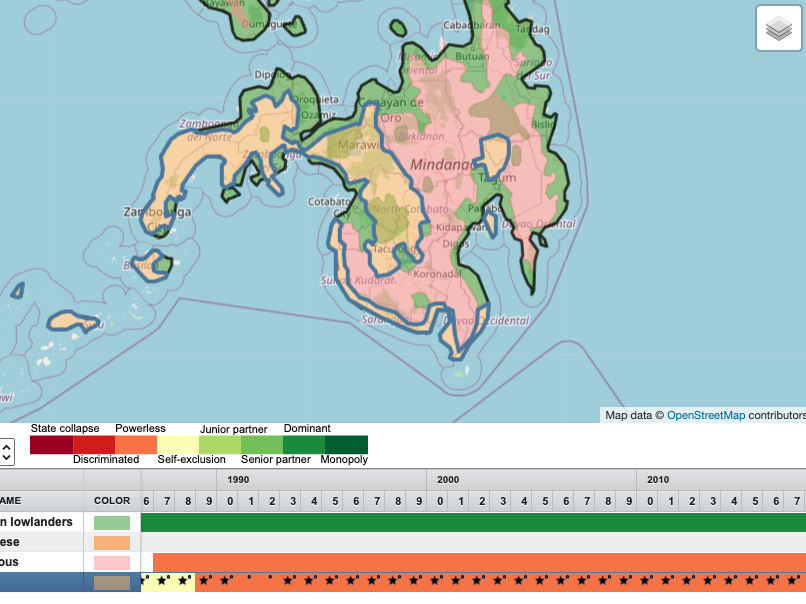
\includegraphics[width = \textwidth]{img/moro_epr}

\end{frame}
% ----------------------------------------------------

% ----------------------------------------------------
\begin{frame}
\frametitle{The role of power-sharing}
\centering

\begin{itemize}[<+->]
  \item A similar problem with a powerful power-sharing device: \BGyellow{democratization}
  \item In principle, it should be good:
  \begin{itemize}
    \item legitimizes postwar governments, gives rebels a platform to seek political goals peacefully, etc
  \end{itemize}
  \item However, particularly if institution are weak, democracy \BGyellow{could be counter-productive}
  \begin{itemize}
    \item Increasing social tensions, polarization, bringing about electoral violence...
    \item Postwar elections might undermine peace if held too son, and democratization during a war might bring about civilian victimization
  \end{itemize}
\end{itemize}

\end{frame}
% ----------------------------------------------------


\end{document}
